\documentclass{standalone}

\usepackage{tikz}

\begin{document}
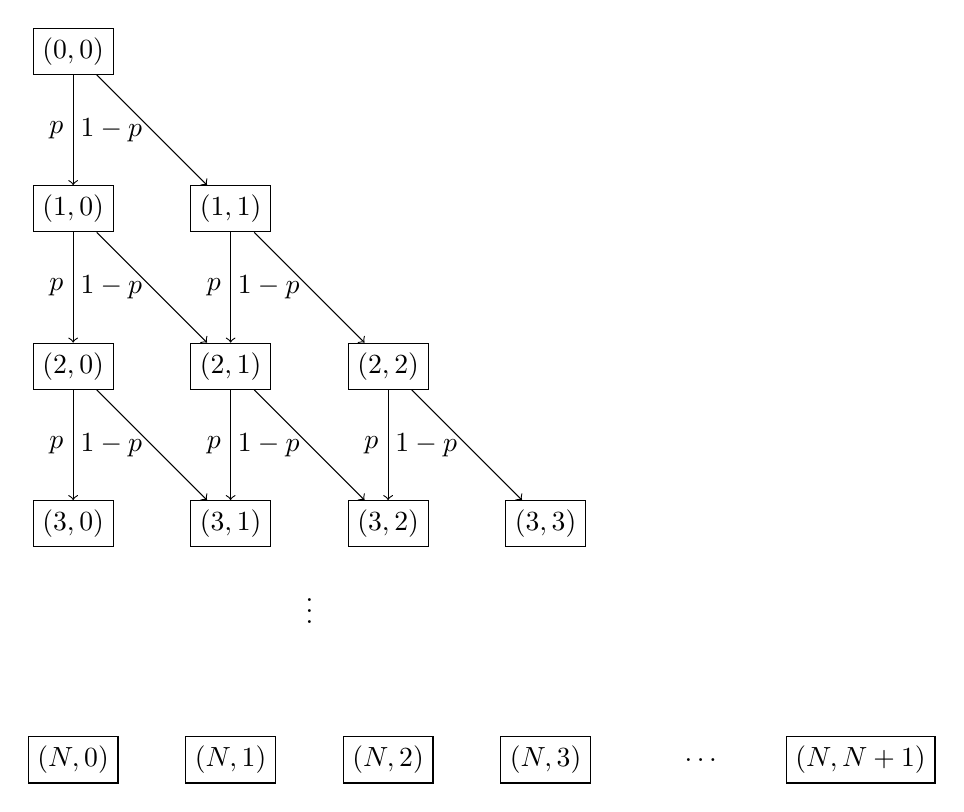
\begin{tikzpicture}
    %\foreach \i \in {0, ..., 4}
        %\foreach \j \in {0, ..., 1}
        %{
            %\node at (\i, \j);
        %}
    \node [draw] (A) at (0, 0) {\((0, 0)\)};


    \node [draw] (B) at (0, -2) {\((1, 0)\)};
    \node [draw] (C) at (2, -2) {\((1, 1)\)};

    \draw [->] (A) -- node [left] {\(p\)} (B);
    \draw [->] (A) -- node [left] {\(1 - p\)} (C);

    \node [draw] (D) at (0, -4) {\((2, 0)\)};
    \node [draw] (E) at (2, -4) {\((2, 1)\)};
    \node [draw] (F) at (4, -4) {\((2, 2)\)};

    \draw [->] (B) -- node [left] {\(p\)} (D);
    \draw [->] (B) -- node [left] {\(1 - p\)} (E);
    \draw [->] (C) -- node [left] {\(p\)} (E);
    \draw [->] (C) -- node [left] {\(1 - p\)} (F);


    \node [draw] (G) at (0, -6) {\((3, 0)\)};
    \node [draw] (H) at (2, -6) {\((3, 1)\)};
    \node [draw] (I) at (4, -6) {\((3, 2)\)};
    \node [draw] (J) at (6, -6) {\((3, 3)\)};

    \draw [->] (D) -- node [left] {\(p\)} (G);
    \draw [->] (D) -- node [left] {\(1 - p\)} (H);
    \draw [->] (E) -- node [left] {\(p\)} (H);
    \draw [->] (E) -- node [left] {\(1 - p\)} (I);
    \draw [->] (F) -- node [left] {\(p\)} (I);
    \draw [->] (F) -- node [left] {\(1 - p\)} (J);

    \node at (3, -7) {\vdots};

    \node [draw] at (0, -9) {\((N, 0)\)};
    \node [draw] at (2, -9) {\((N, 1)\)};
    \node [draw] at (4, -9) {\((N, 2)\)};
    \node [draw] at (6, -9) {\((N, 3)\)};
    \node        at (8, -9) {\dots};
    \node [draw] at (10, -9) {\((N, N + 1)\)};
\end{tikzpicture}
\end{document}
